\documentclass[
	classe=$2^{de}$
]{exercice}

\usepackage{tikz-repère}

\title{Colinéarité et alignement}

\begin{document}

\maketitle

\begin{center}
	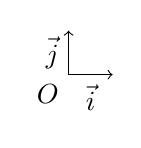
\begin{tikzpicture}[scale=0.56]
		\tikzRepere{-11.5}{11.5}{-9.5}{9.5}[][]
		\node[below left] at (0,0) {$O$};
		\draw[->] (0,0) -- node [below] {$\vec{i}$} (1,0);
		\draw[->] (0,0) -- node [left] {$\vec{j}$} (0,1);

		\ifdefined\makeCorrection
			\coordinate (A) at (2, 1);
			\coordinate (B) at (5, 5);
			\coordinate (C) at (8, 9);
			\coordinate (D) at (-4, -4);
			\coordinate (E) at (-9, -8);

			\foreach \p in {A,B,C,D,E} {
					\node[red] at (\p) {×};
					\node[red,below left] at (\p) {$\p$};
				}
		\fi
	\end{tikzpicture}
\end{center}

\begin{enumerate}
	\item Placer les points $A(2 ; 1)$, $B(5, 5)$ et $C(8, 9)$.
	\item Donner les coordonnées des vecteurs $\vec{AB}\begin{pmatrix}\correction{\ 3\ \ } \\ \correction{4}\end{pmatrix}$ et $\vec{AC}\begin{pmatrix}\correction{\ 6\ \ } \\ \correction{8}\end{pmatrix}$.

	      Les vecteurs $\vec{AB}$ et $\vec{AC}$ sont-ils colinéaires ?

	      \correction{On a $3 × 8 - 4 × 6 = 24 - 24 = 0$.}

	      \correction{Donc les vecteurs $\vec{AB}$ et $\vec{AC}$ sont colinéaires.}
	\item Que peut-on alors dire des points $A$, $B$ et $C$ ?

	      \correction{Ils sont alignés.}
	\item Placer le point $D$, tel que $\vec{AD}\begin{pmatrix}-6 \\ -5\end{pmatrix}$,

	      et le point $E(-9 ; -8)$.
	\item Les points $A$, $D$ et $E$ sont-ils alignés ? Justifier.

	      \correction{Ces points ne sont pas alignés, car les vecteurs $\vec{AD}$ et $\vec{DE}$ ne sont pas colinéaires.}

	      \correction{En effet, on a $\vec{AD}\begin{pmatrix}-6 \\ -5\end{pmatrix}$ et $\vec{DE}\begin{pmatrix}-9 - 3 \\ -8 - 4\end{pmatrix} = \begin{pmatrix}-12 \\ -12\end{pmatrix}$}

	      \correction{Et $-6 × (-12) - (-5) × (-12) = 12 ≠ 0$.}
\end{enumerate}

\end{document}